\begin{figure}
    \centering
    \subfloat[Labeled \& unlabeled interactions]{%
        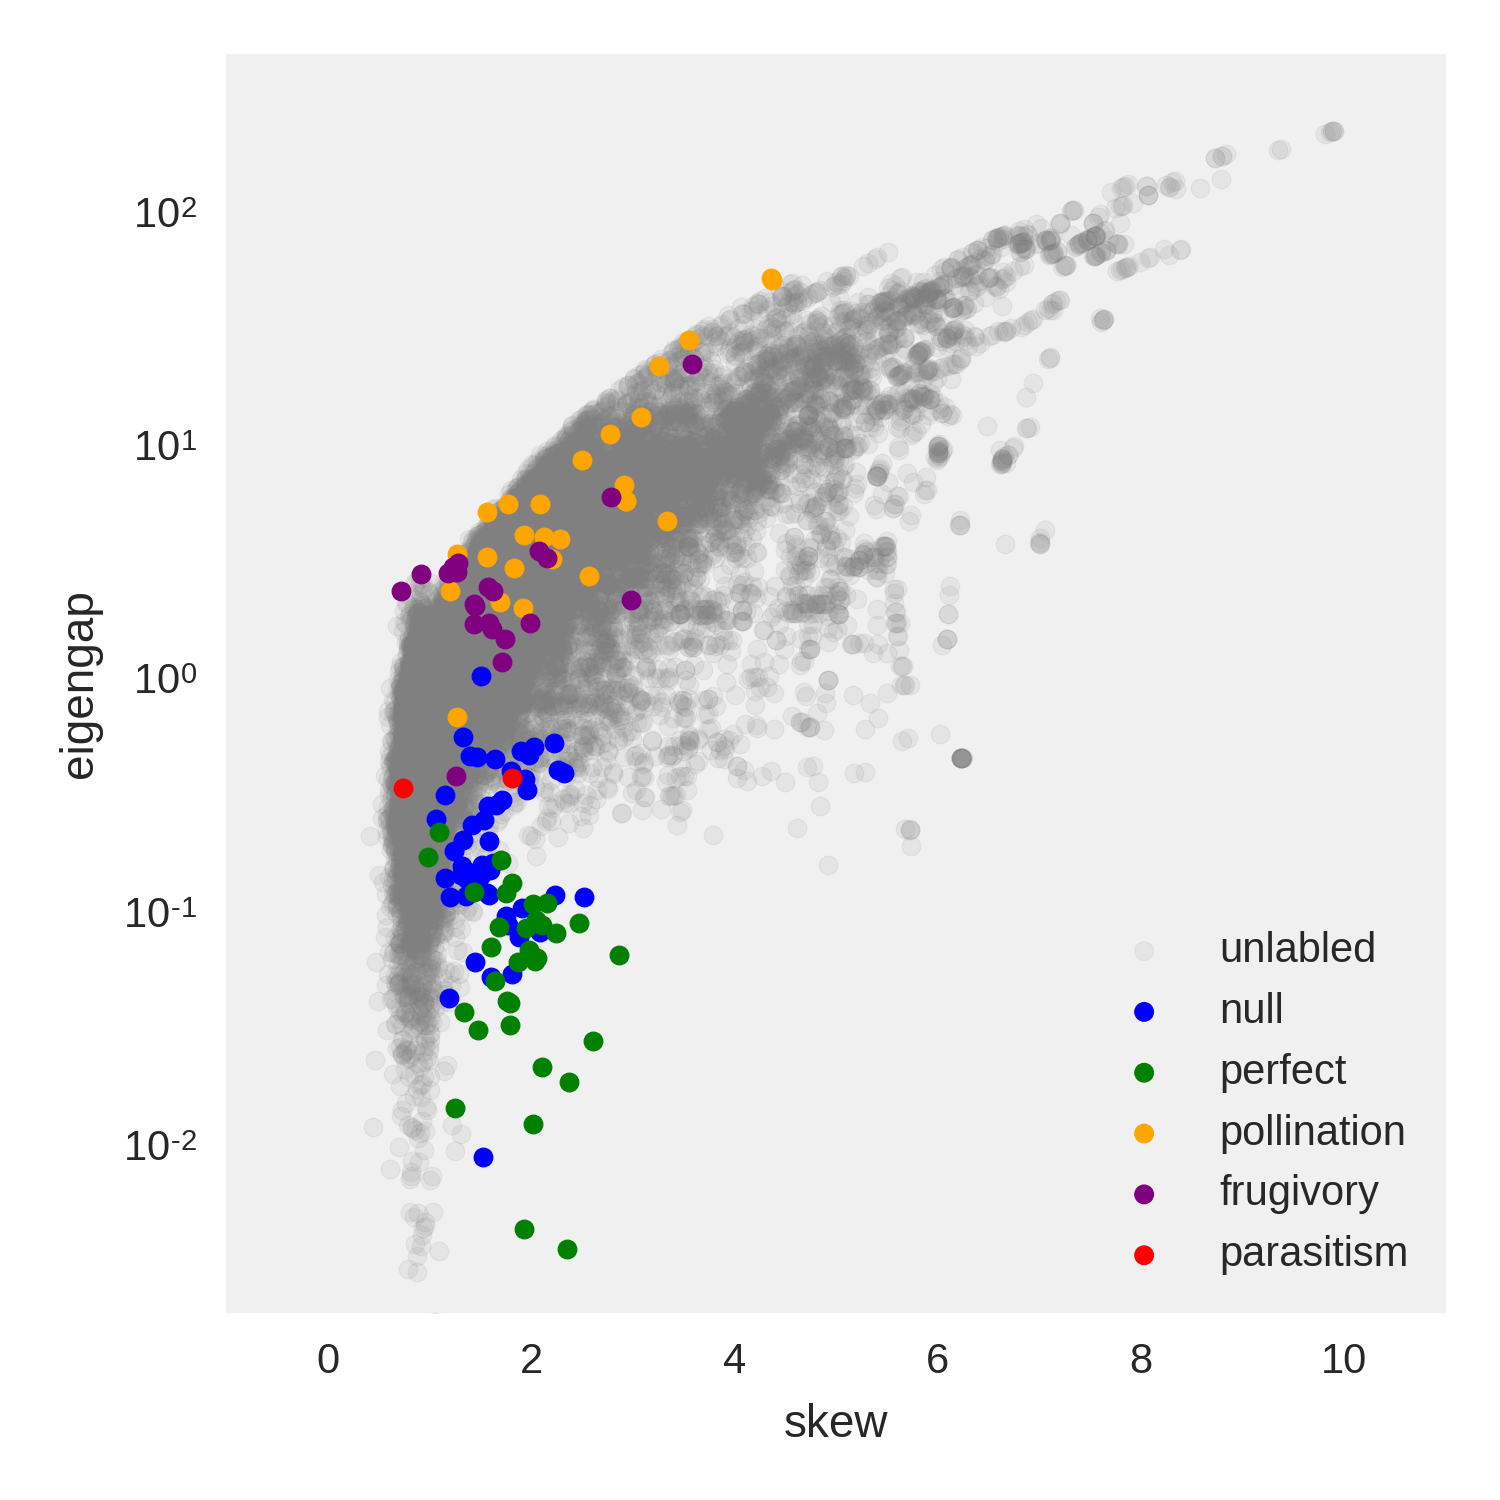
\includegraphics[width=0.5\textwidth]{FishPoo/figures/codiv_literature_fishpoo_classified_skew_eigengap_a.png}
    }
    \subfloat[Classified interactions]{%
        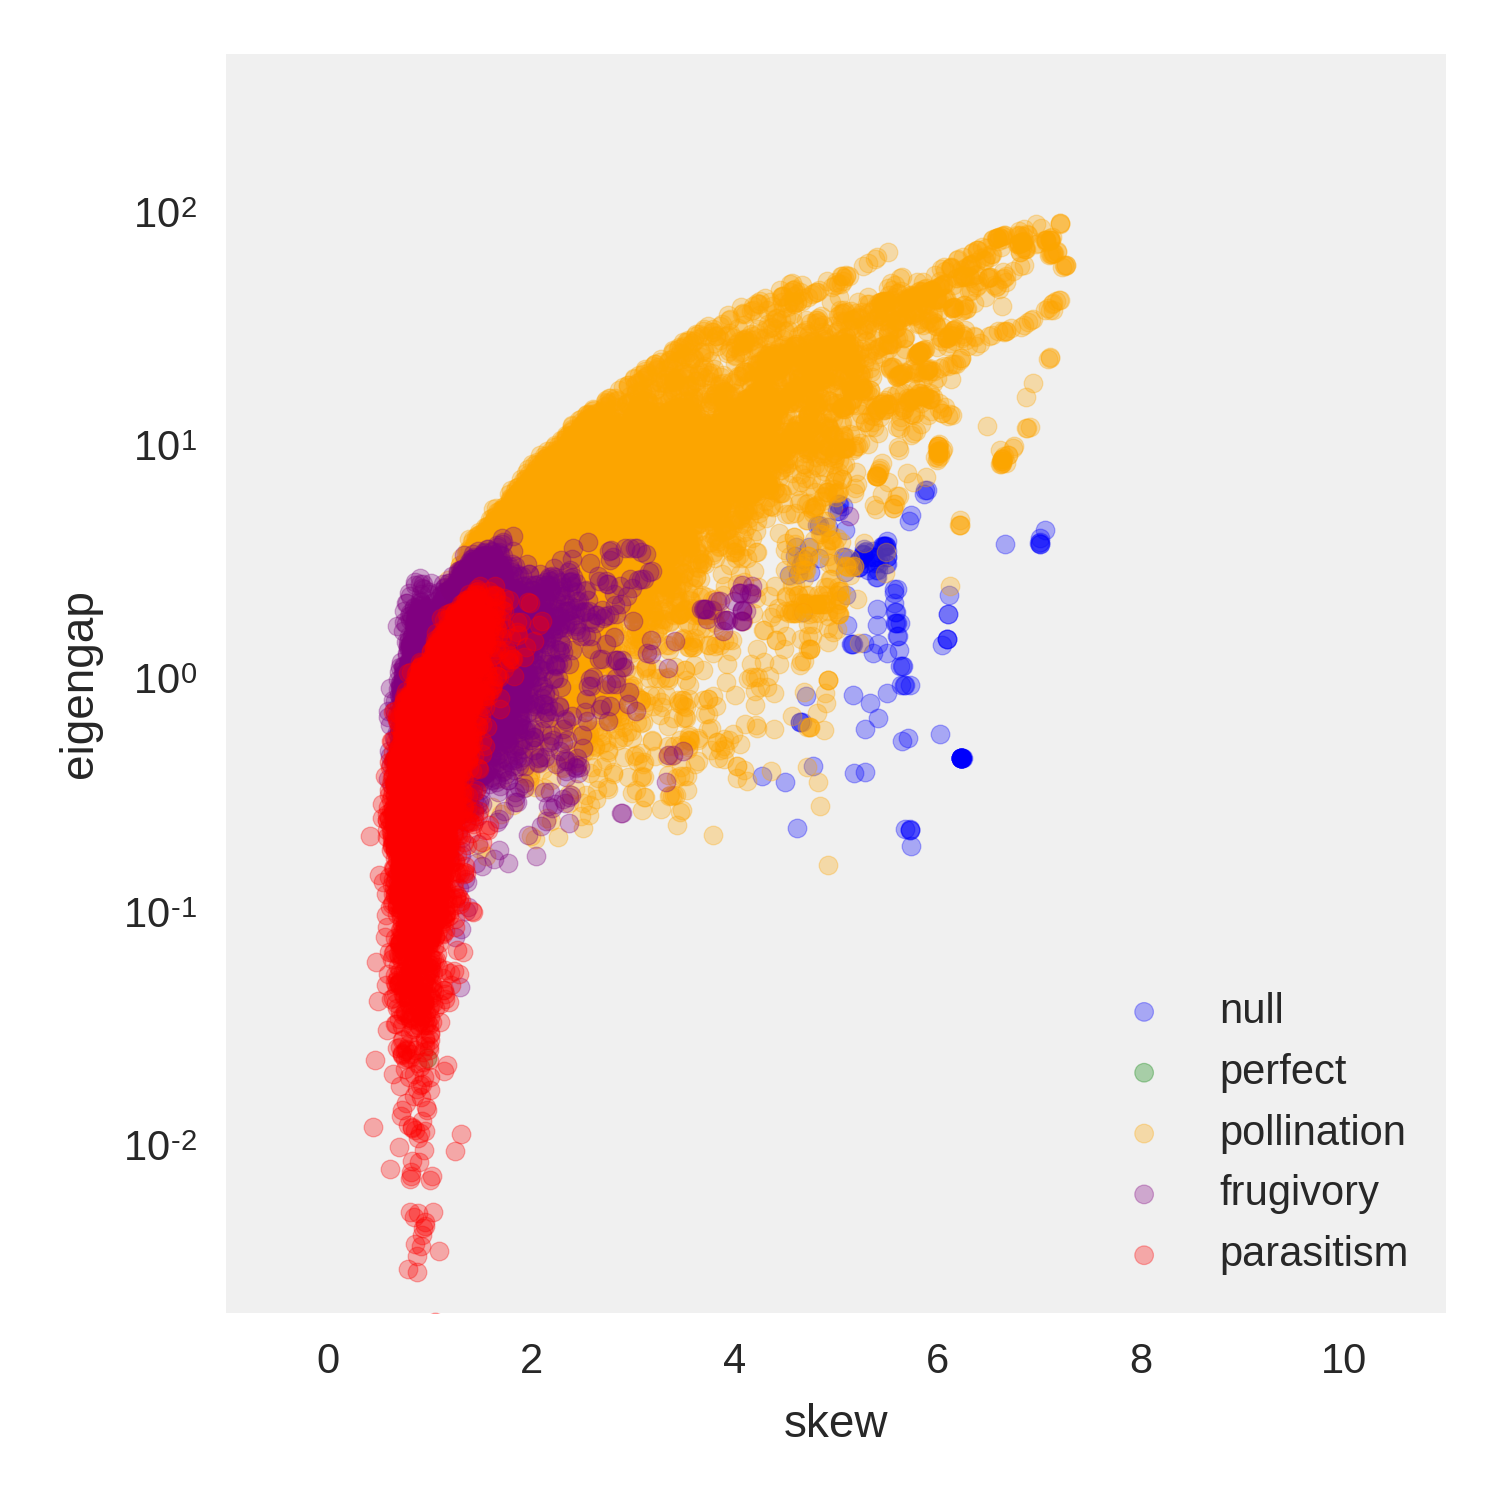
\includegraphics[width=0.5\textwidth]{FishPoo/figures/codiv_literature_fishpoo_classified_skew_eigengap_b.png}
    }\\
    \subfloat[Labeled \& unlabeled interactions]{%
        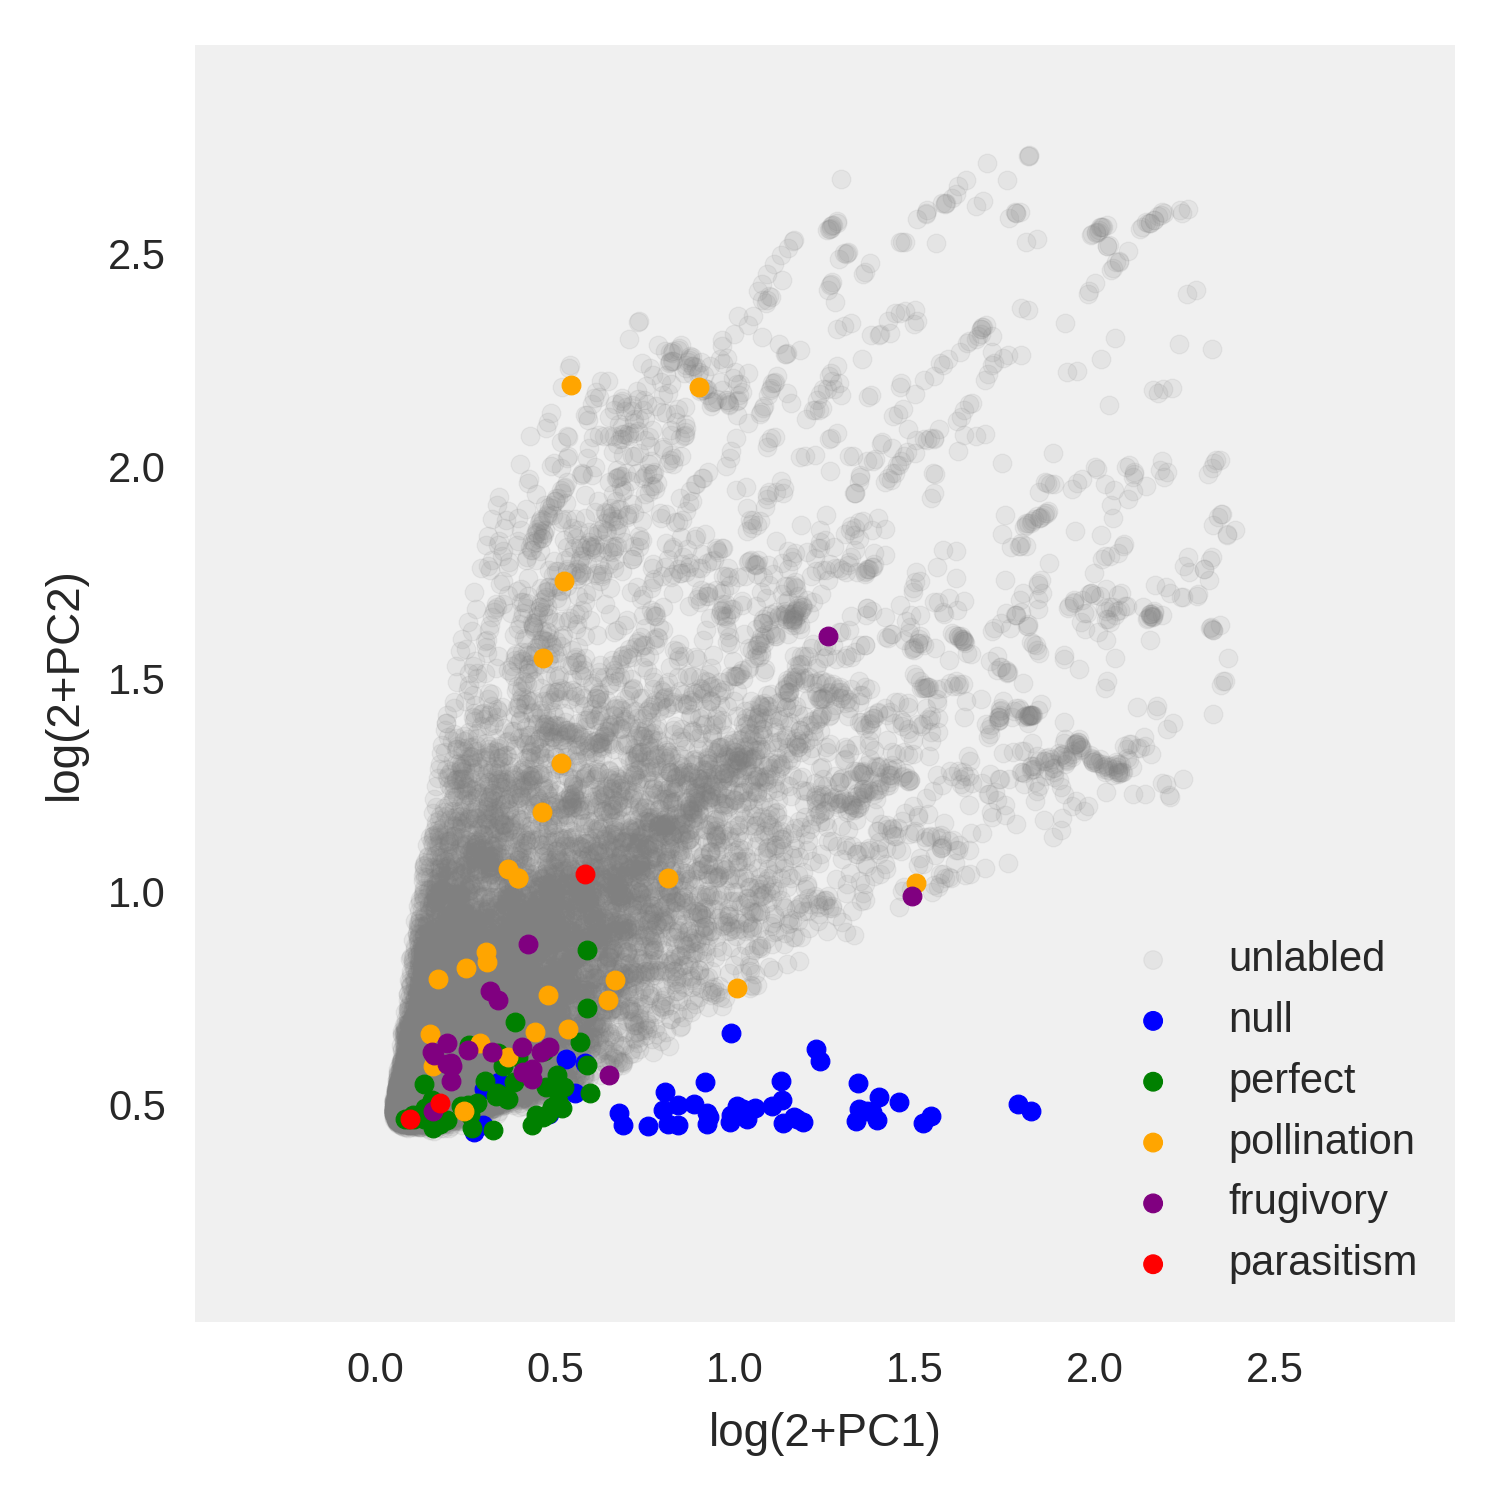
\includegraphics[width=0.5\textwidth]{FishPoo/figures/codiv_literature_fishpoo_classified_PCA_a.png}
    }
    \subfloat[Classified interactions]{%
        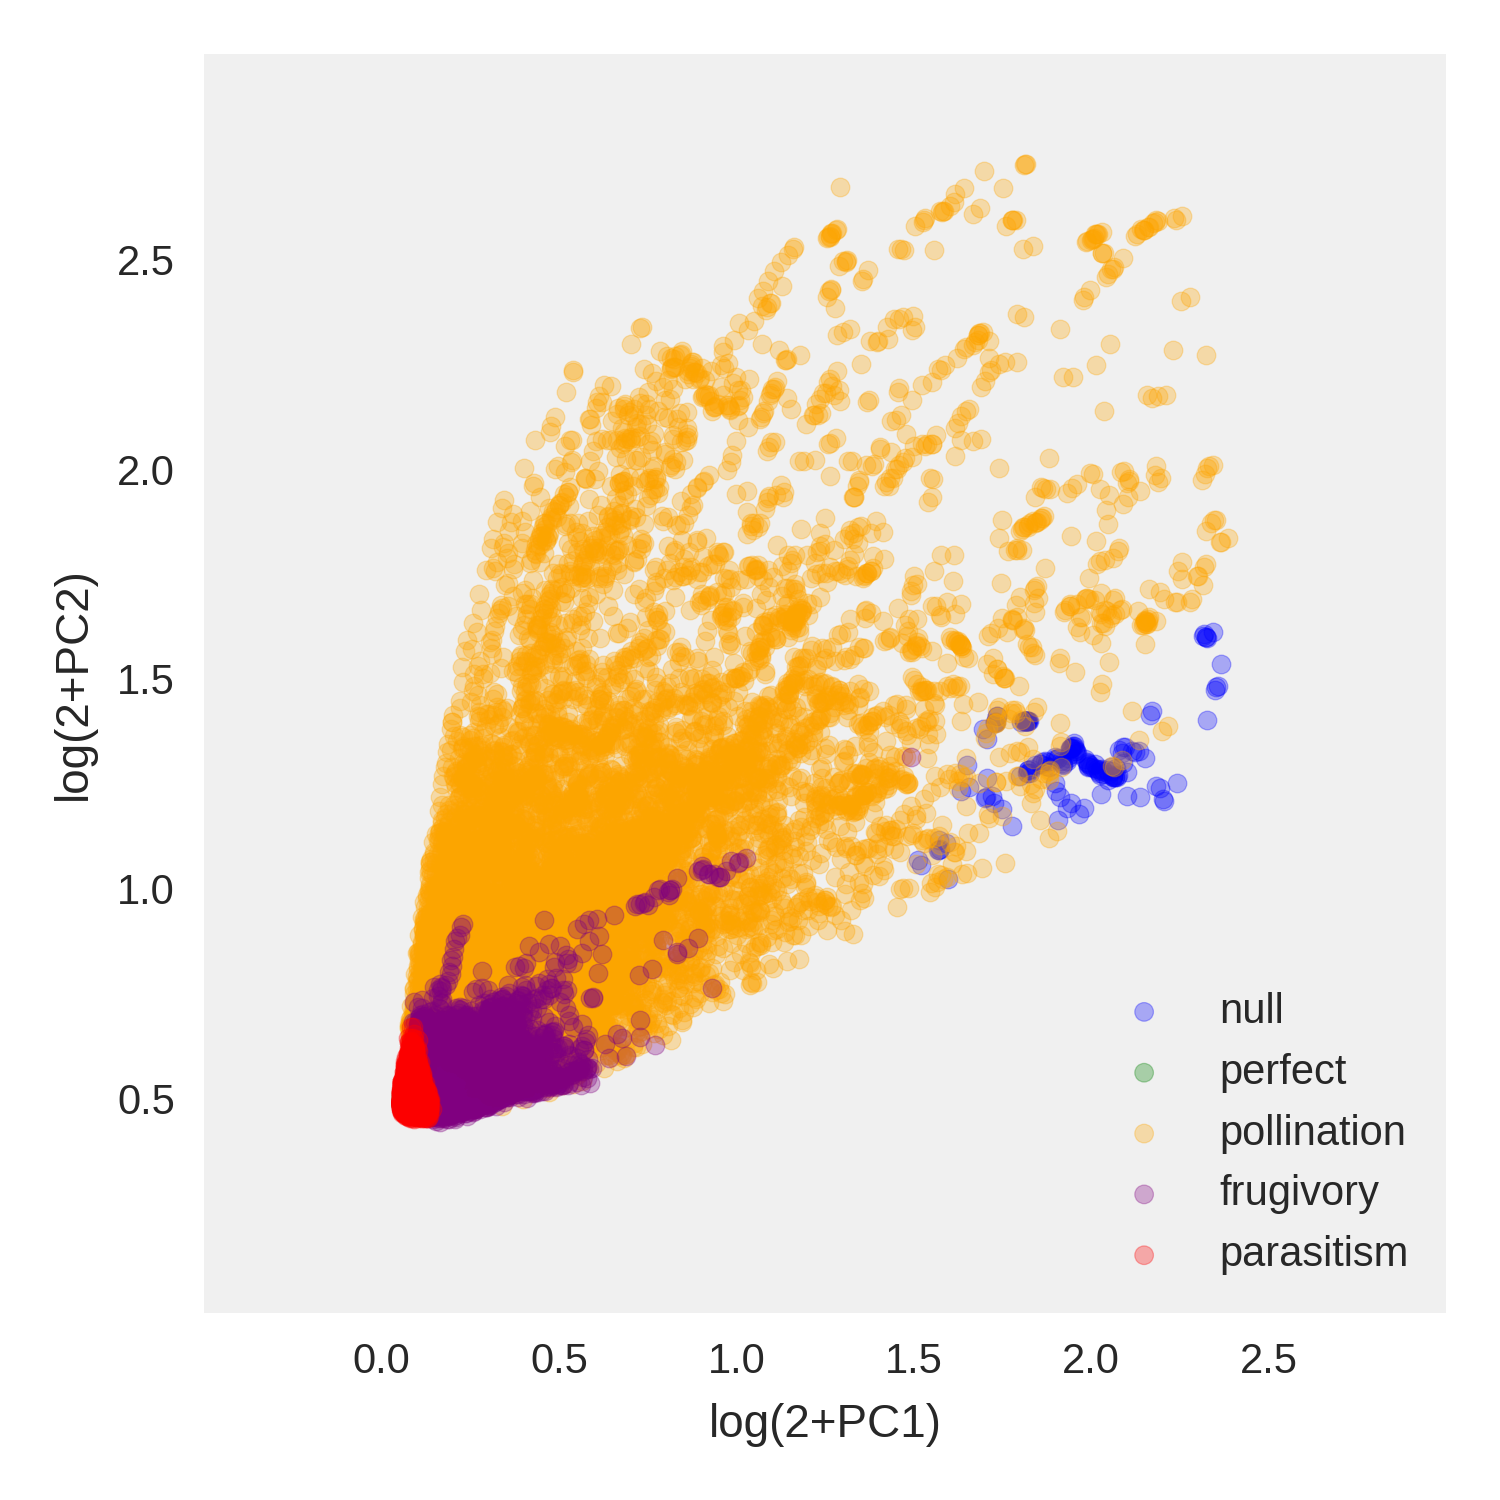
\includegraphics[width=0.5\textwidth]{FishPoo/figures/codiv_literature_fishpoo_classified_PCA_b.png}
    }
    \caption{Projections of labeled and predicted interactions. Projections of unlabeled microbiome interactions and ecological interactions from the literature into subspaces spanned by two important axes of the feature space \textbf{(a)} and the first and second principle components of the feature space of the labeled interactions \textbf{(c)}. A neural network was trained using the feature space of labeled interactions and labels were predicted for the microbiome interactions. These predicted interactions were projected into subspaces spanned by the same two axes of the feature space of labeled interactions \textbf{(b)} and into a space spanned by their first and second principle components \textbf{(d)}.}
    \label{fig:FP_classified}
\end{figure}